Training large language models across geographically distributed datacenters (Cross-DC) introduces system-level challenges that differ fundamentally from those in single-datacenter environments. In particular, Wide Area Networks (WANs) exhibit orders-of-magnitude lower bandwidth, higher latency, and greater variability than intra-datacenter interconnects, fundamentally altering the performance characteristics of distributed training. This section first reviews the design space of Cross-DC training systems and then motivates the design choices underlying this work.

\subsection{Background}

\subsubsection{Cross-Datacenter Training Characteristics}

In Cross-DC settings, compute clusters are interconnected via WAN links that typically provide only 10–30 Gb/s bandwidth with round-trip latencies of 30–100 ms, in stark contrast to intra-datacenter fabrics such as InfiniBand or RDMA-capable Ethernet, which routinely deliver 200–800 Gb/s bandwidth with sub-millisecond latency. These network characteristics fundamentally change the cost model of distributed training: communication that is tolerable within a datacenter can dominate end-to-end iteration time when performed across datacenters. As a result, training systems must tolerate both persistent communication constraints while often operating on geographically partitioned datasets that cannot be easily centralized due to data locality, regulatory, or operational constraints.

\begin{figure}[t]
    \centering
    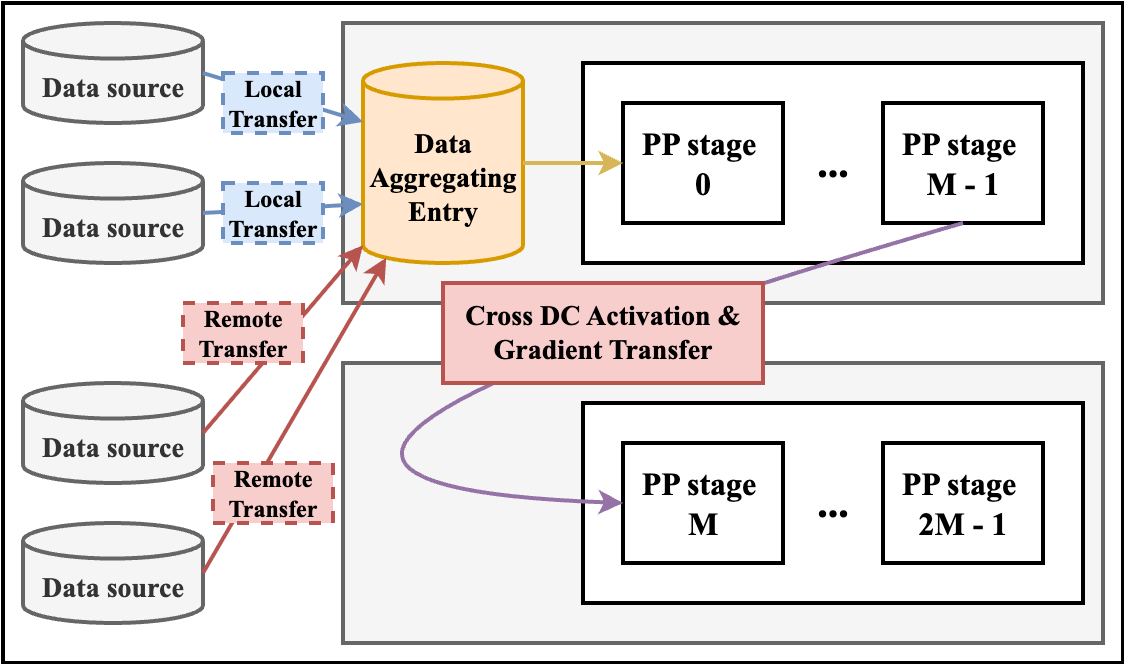
\includegraphics[width=0.96\columnwidth]{images/pp_across_dcs.png}
    \caption{Cross-DC pipeline parallelism. All training data must be aggregated at a single entry-point datacenter, creating severe ingress bottlenecks.}
    \label{fig:cross-dc-pp}
\end{figure}

\begin{figure}[ht]
    \centering
    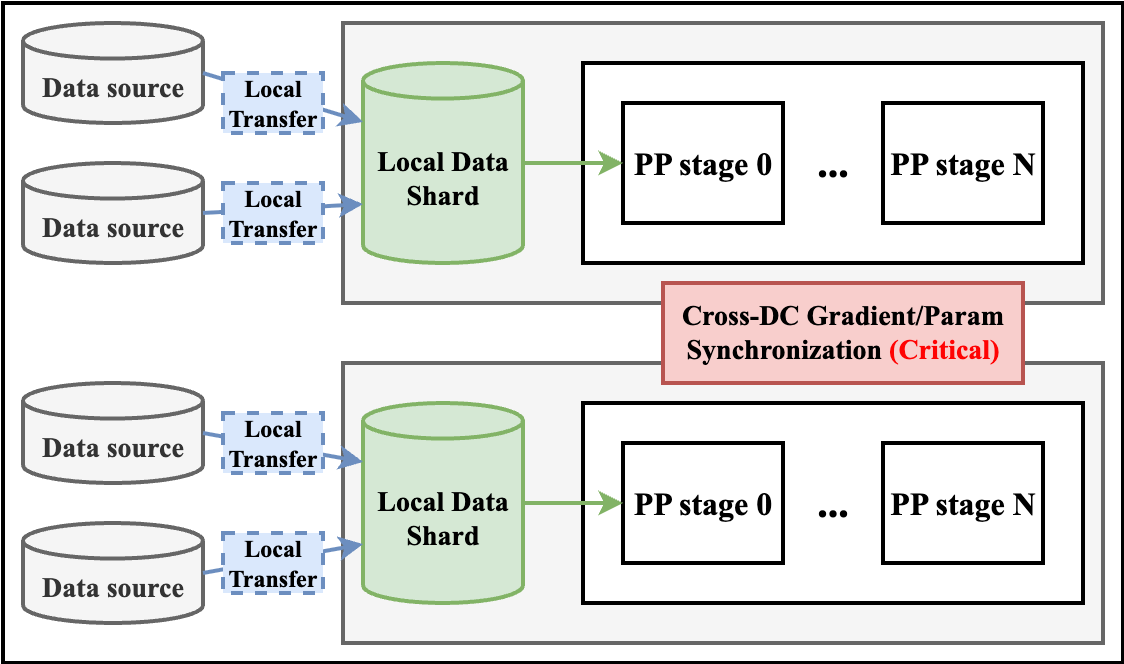
\includegraphics[width=0.96\columnwidth]{images/dp_across_dcs.png}
    \caption{Cross-DC data parallelism with intra-datacenter pipeline parallelism (our setting). Each datacenter processes local data and synchronizes only gradients across the WAN.}
    \label{fig:cross-dc-dp}
\end{figure}

\subsubsection{Parallelism Backbones Indicate a Fundamental Design Trade-off}

To scale training under these constraints, existing Cross-DC systems adopt different parallelism backbones that define how computation and communication are organized across datacenters. Pipeline-parallel–centric designs partition the model into sequential stages and stream micro-batches through the pipeline, enabling training of models that exceed the capacity of individual devices or clusters. Several Cross-DC systems\cite{DBLP:conf/usenix/ChenKHH25, DBLP:journals/corr/abs-2510-12064, DBLP:conf/hotnets/DengS00025} adopt pipeline parallelism as their primary backbone, leveraging its high compute efficiency under ideal communication conditions.

In contrast, data-parallel-centric designs replicate the model across datacenters and partition the dataset instead. Each datacenter performs forward and backward computation locally, while periodically synchronizing model updates across sites. This approach aligns naturally with data locality and minimizes cross-datacenter data movement during the main computation phase, at the cost of explicit synchronization.

\subsubsection{Synchronization and Communication Practices}

Independent of the chosen parallelism backbone, Cross-DC training systems differ in how they synchronize model updates across datacenters. Fully synchronous schemes enforce global barriers at every iteration, preserving strict optimization semantics but exposing WAN latency directly on the training critical path. Asynchronous schemes decouple computation from synchronization, allowing workers to proceed independently, but introduce gradient staleness and potential model divergence. Periodic or local synchronization strategies amortize communication cost by performing multiple local updates before synchronization, trading reduced communication frequency for increased optimization drift.

Collectively, prior work reveals a fundamental tension: synchronization is either frequent and expensive under WAN conditions, or relaxed in ways that perturb the optimization trajectory. This tension motivates a closer examination of how parallelism choices and synchronization interact in Cross-DC environments.

\subsection{Motivation}

\subsubsection{Rethinking Parallelism Choices in Cross-DC Training}
\label{ssb:rethink_parallelism}
Pipeline parallelism is widely regarded as compute-efficient when training is evaluated from a computation-only perspective. By overlapping forward and backward execution across stages, PP can achieve high device utilization under stable, low-latency communication. However, in Cross-DC settings, training efficiency is shaped not only by computation but also by data movement and network dynamics.

In PP-centric Cross-DC designs, training samples or activations must enter the pipeline and be propagated across stages that may span multiple datacenters. Pipeline execution enforces strict ordering constraints between stages, causing delays in cross-datacenter communication to directly stall downstream computation. As illustrated in Figure \ref{fig:cross-dc-pp}, data availability, pipeline progress, and WAN performance become tightly coupled: a slowdown or transient latency spike affecting a single stage can cascade through the pipeline and amplify end-to-end iteration time.

In contrast, data-parallel centric designs localize forward and backward computation within each datacenter. Data loading, preprocessing, and model execution proceed without reliance on WAN communication, and cross-datacenter interaction is confined to synchronization phases outside the main execution path (Figure \ref{fig:cross-dc-dp}). As a result, DP-centric designs are inherently more robust to network variability. 

Our theoretical proofs in the \ref{app:rethink_parallelism} reveal that in scenarios involving training large amounts of data across data centers, the throughput using cross-data center data parallelism is significantly higher than that of cross-data center pipeline parallelism. These observations motivate a hierarchical DP+PP architecture, in which data parallelism is used across data centers to ensure locality and robustness, while pipeline parallelism is employed within each data center to scale model capacity\cite{DBLP:journals/pvldb/KloudasRPM15}.

\subsubsection{Synchronization Becomes the Dominant Bottleneck}

% \begin{figure}[t]
%     \centering
%     \includegraphics[width=0.96\columnwidth]{example-image-duck}
%     \caption{Training flow in DP-based Cross-DC training.}
%     \label{fig:training_flow_dp_based}
% \end{figure}

While a DP+PP backbone addresses data locality and execution robustness, it exposes a new performance bottleneck: cross-datacenter synchronization. In DP-based Cross-DC training, each datacenter independently executes forward and backward passes on local data, but must synchronize model updates to maintain a consistent global model state. 

Under WAN conditions, synchronization latency is no longer negligible. A breakdown of iteration time under a DP+PP configuration (Figure \ref{fig:dppp_timebreakdown}) shows that synchronization in cross-DC scenario can account for a substantial fraction of total iteration time. Consequently, GPUs remain idle for a large fraction of time, waiting for synchronization to complete. 

\begin{figure}[ht]
    \centering
    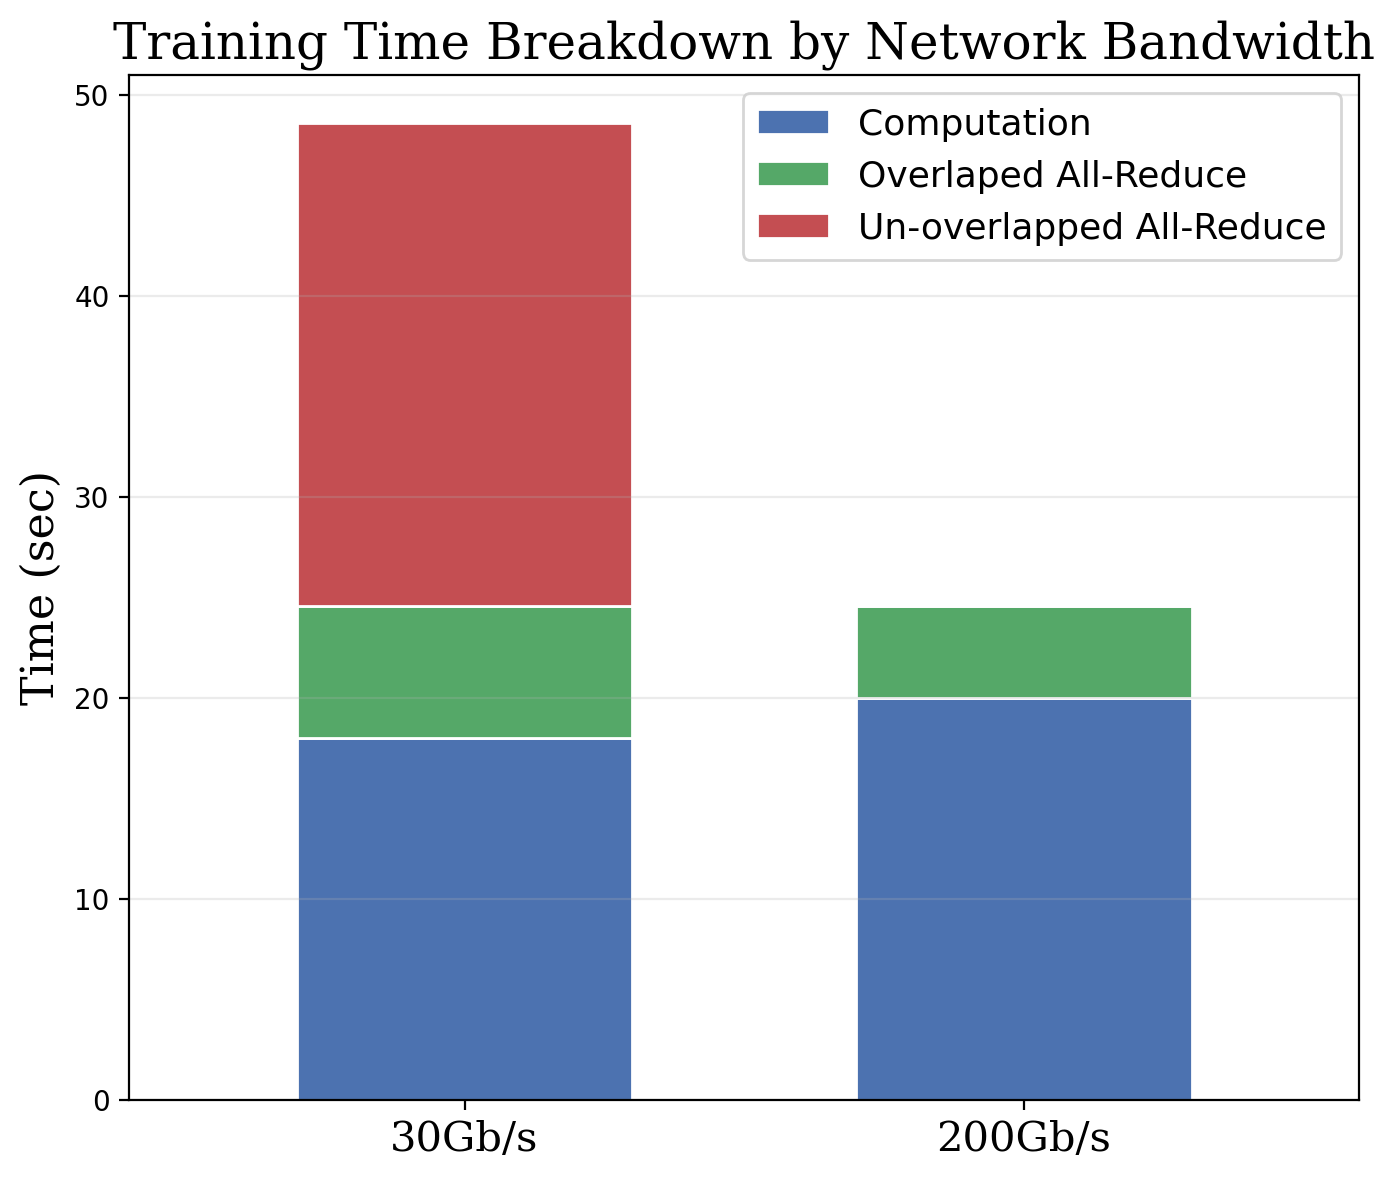
\includegraphics[width=0.96\columnwidth]{images/bar_time_by_network.png}
    \caption{Breakdown of computation and communication overhead per training step under a DP+PP configuration across and within datacenters.}
    \label{fig:dppp_timebreakdown}
\end{figure}



Importantly, existing communication overlap mechanisms in standard data-parallel frameworks\cite{DBLP:journals/pvldb/ZhaoGVLHXWSOSDB23, DBLP:journals/pvldb/LiZVSNLPSVDC20, DBLP:conf/sc/RajbhandariRRH20} only overlap gradient communication within a single backward pass. Under WAN-scale latency, the tail of the synchronization inevitably extends beyond the available computation, making end-of-step blocking unavoidable. Thus, while DP+PP mitigates data-movement inefficiencies, it shifts the primary performance bottleneck to synchronization.


\subsubsection{Decoupling Synchronization Without Sacrificing Optimization Semantics}
A natural response to the synchronization bottleneck is to adopt partially asynchronous methods such as Local-SGD\cite{stich2019local}. However, these schemes exhibit two principal limitations: unresolved performance bottlenecks and an increased risk of model drift during training.\cite{KarimireddyKMRS20, DBLP:conf/iclr/GuLHA23}

From a performance perspective, Local-SGD primarily reduces the frequency of cross-datacenter synchronization rather than eliminating the communication costs inherent to distributed optimization. Periodic global aggregation remains unavoidable. The consequence is sustained GPU idle time.

From an optimization/precision perspective, increasing the number of local steps elevates the risk of model drift. Gradients computed on these stale local replicas introduce systematic bias; this bias can slow convergence and degrade practical generalization performance.

These observations suggest that merely weakening synchronization is insufficient. Conversely, some fully asynchronous schemes\cite{DBLP:journals/corr/abs-2407-07852, DBLP:journals/corr/abs-2501-18512} eliminate compute bubbles but incur severe parameter staleness that is difficult to correct. An effective cross-datacenter training system therefore needs to decouple synchronization from the training critical path while preserving convergence robustness comparable to fully synchronous optimization, rather than relying on strict equivalence of update sequences.


This insight motivates the design of POLAR-SGD.
